\documentclass[border=4pt]{standalone}
\usepackage{tikz}
\usetikzlibrary{positioning, arrows.meta, shapes.geometric, calc, fit, backgrounds}
\usepackage{amsmath,amssymb}
\begin{document}
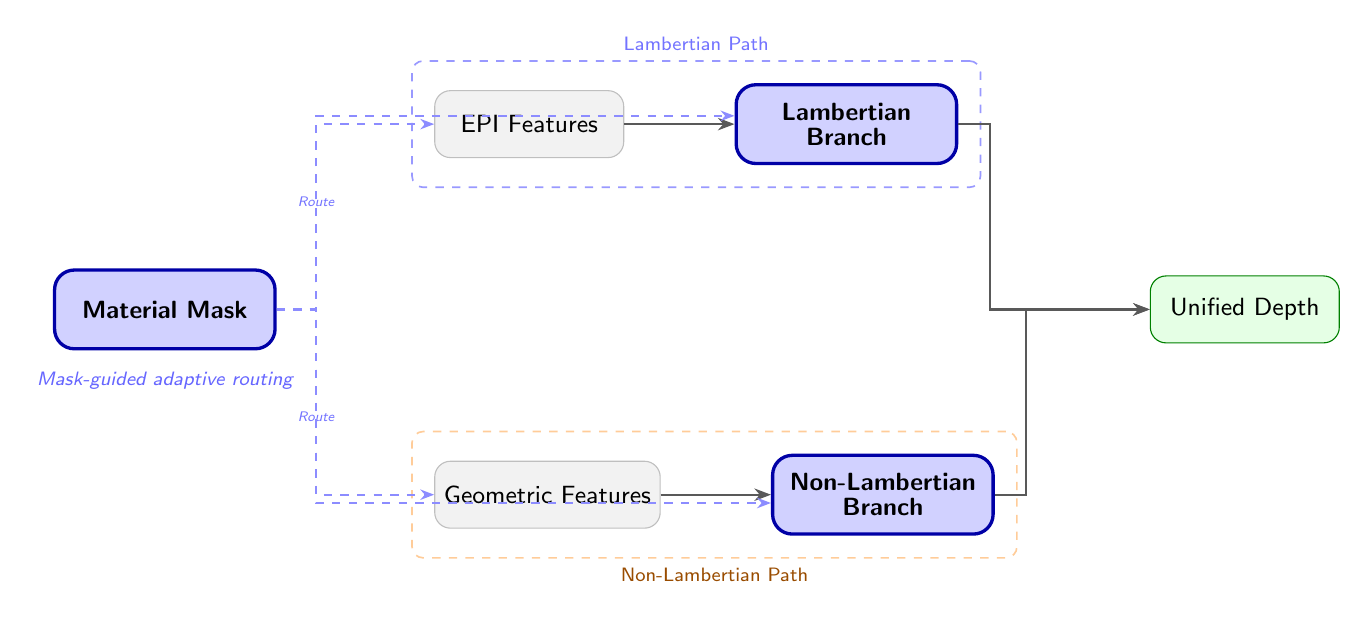
\begin{tikzpicture}[
  % --- Style definitions ---
  input/.style={draw, rounded corners=2mm, minimum width=2.4cm, minimum height=0.85cm,
                fill=gray!10, draw=gray!50, align=center, font=\sffamily\small},
  innov/.style={draw, rounded corners=2.5mm, minimum width=2.8cm, minimum height=1.0cm,
                fill=blue!18, draw=blue!65!black, line width=1.2pt, align=center,
                font=\sffamily\small\bfseries},
  output/.style={draw, rounded corners=2mm, minimum width=2.4cm, minimum height=0.85cm,
                 fill=green!10, draw=green!50!black, align=center, font=\sffamily\small},
  arr/.style={-{Stealth[length=6pt]}, thick, color=black!65},
  arrd/.style={-{Stealth[length=5pt]}, thick, dashed, color=blue!45},
  lbl/.style={font=\sffamily\scriptsize, text=black!45, fill=white, inner sep=1pt},
  gbox/.style={draw=#1, dashed, rounded corners=4pt, inner sep=8pt, line width=0.6pt},
  ann/.style={font=\sffamily\tiny\itshape, text=blue!55},
]

% ===== Nodes =====

% --- Column 1: Material Mask (centered vertically) ---
\node[innov] (m1) {Material Mask};

% --- Column 2: Input features (top and bottom) ---
\node[input, above right=1.4cm and 2.0cm of m1] (m2) {EPI Features};
\node[input, below right=1.4cm and 2.0cm of m1] (m4) {Geometric Features};

% --- Column 3: Branch modules (top and bottom) ---
\node[innov, right=1.4cm of m2] (m3) {Lambertian\\[-2pt]Branch};
\node[innov, right=1.4cm of m4] (m5) {Non-Lambertian\\[-2pt]Branch};

% --- Column 4: Unified output (centered vertically) ---
\coordinate (merge) at ($(m3.east)!0.5!(m5.east)$);
\node[output, right=2.2cm of merge] (m6) {Unified Depth};

% ===== Grouping boxes (background) =====
\begin{scope}[on background layer]
  \node[gbox=blue!40, fit=(m2)(m3),
        label={[font=\sffamily\scriptsize, text=blue!55]above:Lambertian Path}] (g1) {};
  \node[gbox=orange!40, fit=(m4)(m5),
        label={[font=\sffamily\scriptsize, text=orange!60!black]below:Non-Lambertian Path}] (g2) {};
\end{scope}

% ===== Arrows =====

% Main data flow: inputs to branches
\draw[arr] (m2) -- (m3);
\draw[arr] (m4) -- (m5);

% Branches to output
\draw[arr] (m3.east) -- ++(0.4,0) |- (m6.west);
\draw[arr] (m5.east) -- ++(0.4,0) |- (m6.west);

% Routing arrows from Material Mask
\draw[arrd] (m1.east) -- ++(0.5,0) |- node[ann, pos=0.25, above] {Route} (m2.west);
\draw[arrd] (m1.east) -- ++(0.5,0) |- node[ann, pos=0.25, below] {Route} (m4.west);

% Routing arrows from Material Mask to branches (secondary routing)
\draw[arrd] (m1.east) -- ++(0.5,0) |- ([yshift=3pt]m3.west);
\draw[arrd] (m1.east) -- ++(0.5,0) |- ([yshift=-3pt]m5.west);

% ===== Key annotation =====
\node[ann, text=blue!60, font=\sffamily\scriptsize\itshape,
      below=0.15cm of m1] {Mask-guided adaptive routing};

\end{tikzpicture}
\end{document}